%\documentclass[12pt, twoside]{book}
\documentclass[12pt, oneside]{book}  % jednostranna tlac

%spravne nastavenie okrajov
\usepackage[a4paper,top=2.5cm,bottom=2.5cm,left=3.5cm,right=2cm]{geometry}
%zapnutie fontov pre UTF8 kodovanie
\usepackage[utf8]{inputenc}
\usepackage[T1]{fontenc}

%zapnutie slovenskeho delenia slov
%a automatickych nadpisov ako Obsah, Obrázok a pod. v slovencine
\usepackage[slovak]{babel} % vypnite pre prace v anglictine!

%nastavenie riadkovania podla smernice
\linespread{1.25} % hodnota 1.25 by mala zodpovedat 1.5 riadkovaniu

% balicek na vkladanie zdrojoveho kodu
\usepackage{listings}
% ukazky kodu su cislovane ako Listing 1,2,...
% tu je Listing zmenene na Algoritmus 1,2,...
\renewcommand{\lstlistingname}{Algoritmus}
% nastavenia balicka listings
% mozete pridat aj language=...
% na nastavenie najcastejsie pouzivaneho prog. jazyka
% takisto sa da zapnut cislovanie riadkov
\lstset{frame=lines}

% balicek na vkladanie obrazkov
\usepackage{graphicx}
% balicek na vkladanie celych pdf dokumentov, tu zadanie
\usepackage{pdfpages}
% balicek na spravne formatovanie URL
\usepackage{url}
% balicek na hyperlinky v ramci dokumentu
% zrusime farebne ramiky okolo liniek aby pdf
% vyzeralo rovnako ako tlacena verzia
\usepackage[hidelinks,breaklinks]{hyperref}

% balicek pre matematicke prostredia a vyrazy
\usepackage{amsmath}

% prikaz \uv pre slovenske uvodzovky („...“)
% (niektore verzie babel ho definuju samy, preto \providecommand)
\providecommand{\uv}[1]{\quotedblbase #1\textquotedblleft}


% -------------------
% --- Definicia zakladnych pojmov
% --- Vyplnte podla vasho zadania, rok ma byt rok odovzdania
% -------------------
\def\mfrok{2027}
\def\mfnazov{Návrh a implementácia nástroja na softvérovú inventúru a identifikáciu zraniteľností}
\def\mftyp{Diplomová práca}
\def\mfautor{Bc. Tibor Černák}
\def\mfskolitel{prof. RNDr. Roman Ďurikovič, PhD.}

%ak mate konzultanta, odkomentujte aj jeho meno na titulnom liste
\def\mfkonzultant{Ing. Peter Pištek, PhD.}

\def\mfmiesto{Bratislava, \mfrok}

% údaje podľa zadania z AIS2
\def\mfodbor{ informatika }
\def\program{ Aplikovaná informatika }

% Ak je školiteľ z FMFI, uvádzate katedru školiteľa, zrejme by mala byť aj na zadaní z AIS2
% Ak máte externého školiteľa, uvádzajte Katedru informatiky
\def\mfpracovisko{ Katedra aplikovanej informatiky }

\begin{document}
\frontmatter
\pagestyle{empty}

% -------------------
% --- Obalka ------
% -------------------

\begin{center}
\sc\large
Univerzita Komenského v Bratislave\\
Fakulta matematiky, fyziky a informatiky

\vfill

{\LARGE\mfnazov}\\
\mftyp
\end{center}

\vfill

{\sc\large
\noindent \mfrok\\
\mfautor
}

\cleardoublepage
% --- koniec obalky ----

% -------------------
% --- Titulný list
% -------------------


\noindent

\begin{center}
\sc
\large
Univerzita Komenského v Bratislave\\
Fakulta matematiky, fyziky a informatiky

\vfill

{\LARGE\mfnazov}\\
\mftyp
\end{center}

\vfill

\noindent
\begin{tabular}{ll}
Študijný program: & \program \\
Študijný odbor: & \mfodbor \\
Školiace pracovisko: & \mfpracovisko \\
Školiteľ: & \mfskolitel \\
Konzultant: & \mfkonzultant \\
\end{tabular}

\vfill


\noindent \mfmiesto\\
\mfautor

\cleardoublepage
% --- Koniec titulnej strany


% -------------------
% --- Zadanie z AIS
% -------------------
% v tlačenej verzii s podpismi zainteresovaných osôb.
% v elektronickej verzii sa zverejňuje zadanie bez podpisov
% v pracach v angličtine anglické aj slovenské zadanie

\newpage
\setcounter{page}{3}
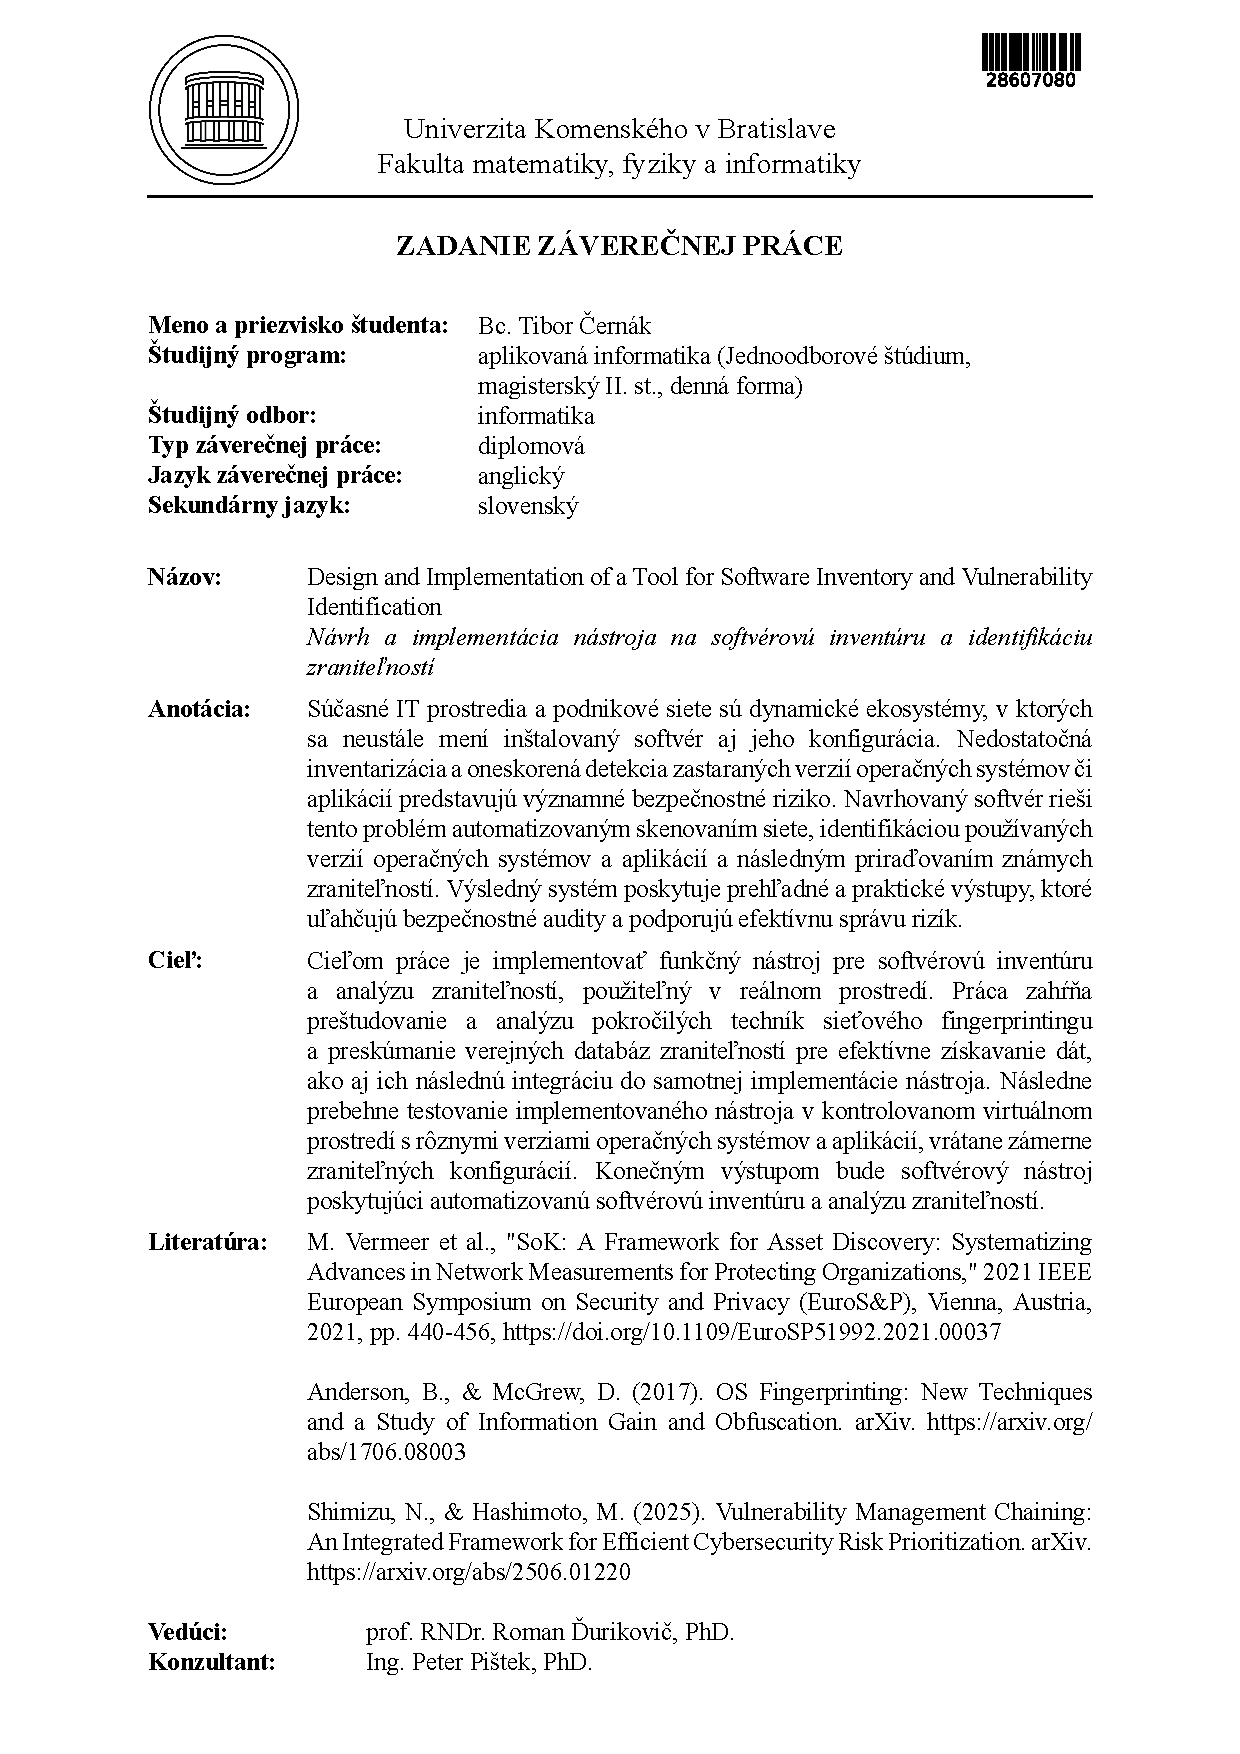
\includepdf{images/zadanie.pdf}

% --- Koniec zadania


% -------------------
%   Čestné vyhlásenie a nepovinné poďakovanie
% -------------------
\newpage
\pagestyle{plain}
\paragraph{Čestné vyhlásenie:}
Čestne vyhlasujem, že celú diplomovú prácu na tému \uv{\mfnazov},
vrátane všetkých jej príloh a obrázkov, som vypracoval
samostatne, a to s použitím literatúry uvedenej v priloženom zozname.

% Uveďte na čo ste nástroje používali
% Podľa typu použitia potom nástroje aj citujte v texte
Pri príprave tejto práce boli tiež použité nástroje umelej
inteligencie [ZOZNAM NÁSTROJOV] za účelom [DÔVOD]. Nástroje umelej
inteligencie som použil v súlade s príslušnými právnymi
predpismi, akademickými právami a slobodami, etickými a morálnymi
zásadami za súčasného dodržania akademickej integrity. Som si
vedomý, že plne zodpovedám za správnosť výsledného textu.

\paragraph{Poďakovanie:} Tu môžete poďakovať školiteľovi, prípadne
ďalším osobám, ktoré vám s prácou nejako pomohli, poradili,
poskytli dáta a podobne.

% --- Koniec poďakovania

% -------------------
%   Abstrakt - Slovensky
% -------------------
\newpage
\section*{Abstrakt}


Slovenský abstrakt v rozsahu 100-500 slov, jeden odstavec. Abstrakt
stručne sumarizuje výsledky práce. Mal by byť pochopiteľný pre bežného
informatika. Nemal by teda využívať skratky, termíny alebo označenie
zavedené v práci, okrem tých, ktoré sú všeobecne známe.

\paragraph*{Kľúčové slová:} jedno, druhé, tretie (prípadne štvrté, piate)
% --- Koniec Abstrakt - Slovensky


% -------------------
% --- Abstrakt - Anglicky
% -------------------
\newpage
\section*{Abstract}

Abstract in the English language (translation of the abstract in the
Slovak language).


\paragraph*{Keywords:}

% --- Koniec Abstrakt - Anglicky

% -------------------
% --- Obsah
% -------------------


\cleardoublepage
\tableofcontents

% ---  Koniec Obsahu

% -------------------
% --- Zoznamy tabuliek, obrázkov, skratiek, slovník - nepovinné
% -------------------

\newpage

\listoffigures
\listoftables

% ---  Koniec Zoznamov

\mainmatter
\pagestyle{headings}


\chapter*{Úvod} % chapter* je necislovana kapitola
\addcontentsline{toc}{chapter}{Úvod} % rucne pridanie do obsahu
\markboth{Úvod}{Úvod} % vyriesenie hlaviciek


\chapter{Súčasný stav riešenej problematiky}
\label{kap:sucasnyStav}

\section{Správa zraniteľností}
\label{sec:spravaZranitelnosti}

Súčasné organizácie prevádzkujú veľké množstvo zariadení, v ktorých sa inštalovaný softvér a jeho konfigurácia neustále mení.
Táto dynamika je ešte viac posilnená zmenami v prostredí zraniteľností, kde sú nové zraniteľnosti objavované a verejne zverejňované denne.
Nedostatočná inventarizácia a oneskorená detekcia zraniteľných verzií softvéru môže predstavovať významné bezpečnostné riziko.

Správa zraniteľností preto nie je jednorazovou činnosťou, ale nepretržitým cyklom zberu údajov, analýzy, prioritizácie, nápravy a overenia.

Zber údajov v prvom kroku rozdeľujeme na interný a externý. Interný zber údajov zahŕňa zhromažďovanie informácií o prostredií organizácie,
čo predstavuje informácie o pripojených zariadeniach v sieti, ich operačnom systéme, nainštalovanom softvéri 
a jeho verziach a pri použití niektorých nástrojov na detekciu zraniteľností aj o konkrétnych zraniteľnostiach.
Externý zber údajov zahŕňa získavanie informácií o zraniteľnostiach z verejne dostupných zdrojov.
Keďže oba typy údajov rýchlo prestávajú byť aktuálne, je potrebné zber vykonávať pravidelne.

Pri analýze porovnávame zozbieraný inventár so známymi zraniteľnosťami s cieľom určiť, ktoré zariadenia sú zraniteľné. 
Keďže počet nájdených zraniteľností pri jednotlivých zariadeniach môže dosahovať aj desiatky či stovky a zdroje na ich
odstránenie sú limitované, je potrebná ich prioritizácia, pri ktorej sa zohľadňuje aktívne zneužívanie v praxi a kritickosť daného aktíva pre prevádzku.

Utriedené zraniteľnosti následne odstraňujeme prostredníctvom aktualizácií alebo v prípadoch, keď oprava nie je dostupná,
dočasným zmiernením rizika. 
Na záver overujeme, či boli riešené zraniteľnosti úspešne odstránené, a zároveň získavame informácie o nových zraniteľnostiach,
čím sa celý cyklus začína odznova.

\section{Identifikácia a hodnotenie zraniteľností}
\label{sec:identifikaciaHodnotenie}

Kvôli potrebe jednotnej identifikácie zraniteľností naprieč rôznymi nástrojmi a databázmi vznikol systém CVE (Common Vulnerabilities and Exposures), 
ktorý slúži ako štandardizovaný systém na označovanie známych bezpečnostných zraniteľností. 
S narastajúcim množstvom zraniteľností bolo potrebné určiť aj ich závažnosť, aby sa uprednostnili kritickejšie. Na tento účel vznikol
systém CVSS (Common Vulnerability Scoring System), ktorý hodnotí závažnosť zraniteľnosti číselným skóre. 
Neskôr tento systém doplnili aj iné ukazovatele, CISA KEV (Known Exploited Vulnerabilities) a EPSS (Exploit Prediction Scoring System)


\subsection{Identifikácia zraniteľností}
\label{subsec:identifikaciaZranitelnosti}
\subsubsection*{CVE}
Výskumná a vývojová organizácia financovaná vládou USA, The MITRE Corporation, vyvinula v roku 1999 systém CVE. 
Každej verejne známej zraniteľnosti v oblasti informačnej bezpečnosti je priradený jednoznačný identifikátor 
CVE Identifier (tiež známy ako CVE ID), ktorý má tvar CVE-YYYY-XXXX, kde YYYY je rok zverejnenia a XXXX je číslo 
pozostávajúce zo štyroch (alebo viac) číslic. Záznamy CVE sú stručné, obsahujú krátky opis, dotknuté produkty a referencie.
Bližšie informácie o rizikách, dôsledkoch, referencie na opravy a hodnotení závažnosti zraniteľností sa nachádzajú v iných
databázach, z ktorých najznámejšia je National Vulnerability Database (NVD).
CVE číslovacia autorita (CVE Numbering Authority - CNA) je organizácia oprávnená prideľovať CVE 
identifikátory a zabezpečuje vytvorenie a zverejnenie informácií o zraniteľnosti v danom zázname CVE.
V čase písania tejto práce existuje vyše 500 CNA, pozostávajúcich z bezpečnostných spoločností, výskumných organizácií a dodávateľov
softvéru a hardvéru, ako Microsoft, Apple, Cisco a pod. \cite{cvePartners}. Na Slovensku pôsobia tri organizácie s rolou CNA, z ktorých za zmienku 
stoja Národné centrum kybernetickej bezpečnosti SK-CERT a spoločnosť ESET. Každá CNA dostáva blok identifikátorov CVE,
ktoré následne priraďuje k novoobjaveným zraniteľnostiam v rámci svojej pôsobnosti.

\subsubsection*{CPE}

Zatiaľ čo samotný záznam CVE hovorí o existencii zraniteľnosti, CPE (Common Platform Enumeration) slúži na jednoznačné 
určenie produktu a jeho verzie, ktoré sú zraniteľnosťou zasiahnuté.
CPE je štrukturovaný systém pomenúvania na jednoznačnú identifikáciu softvéru, operačných systémov, hardvéru, spravovaný
organizáciou NIST (The National Institute of Standards and Technology).

Formát CPE vyzerá nasledovne \cite{cheikes2011cpe23}:
\begin{verbatim}
  cpe:cpe_version:part:vendor:product:version:update:edition:language:
  sw_edition:target_sw:target_hw:other
\end{verbatim}
kde 
\begin{itemize}
    \item \texttt{cpe\_version} - verzia CPE, najnovšia verzia je 2.3.
    \item \texttt{part} - typ produktu: \texttt{a} (aplikácia), \texttt{o} (operačný systém), \texttt{h} (hardvér).
    \item \texttt{vendor} - názov výrobcu alebo dodávateľa produktu.
    \item \texttt{product} - názov produktu.
    \item \texttt{version} - verzia produktu.
    \item \texttt{update} - konkrétna aktualizácia alebo záplata.
    \item \texttt{edition} - edícia produktu (v CPE 2.3 zastarané).
    \item \texttt{language} - jazyk produktu podľa IETF RFC 5646 (napr. \texttt{en-US}, \texttt{sk-SK}).
    \item \texttt{sw\_edition} - špecifické vydanie pre konkrétny trh (napr. \texttt{pro}, \texttt{community}).
    \item \texttt{target\_sw} - špecifikácia softvérového prostredia, v ktorom produkt beží.
    \item \texttt{target\_hw} - špecifikácia hardvéru, na ktorom produkt beží (napr. \texttt{x86}).
    \item \texttt{other} - doplňujúce informácie.
\end{itemize}
V reťazci sa môžu vyskytovať aj zástupné hodnoty (wildcard character) \texttt{*} označujúce ľubovoľnú hodnotu a \texttt{-} označujúce nepoužiteľné pole.
Príklad CPE 2.3 pre aplikáciu 7-zip s verziou 3.13 pre Windows:
\begin{verbatim}
    cpe:2.3:a:7-zip:7-zip:3.13:*:*:*:*:windows:*:*
\end{verbatim}

Identifikátory CPE sú verejne dostupné v oficiálnom slovníku CPE (CPE Dictionary), ktorý
spravuje už spomínaný NIST v rámci databázy NVD (National Vulnerability Database).
V praxi pri správe zraniteľností sa po vygenerovaní zoznamu nainštalovaného softvéru a jeho verzií tento softvér najprv 
namapuje na zodpovedajúce identifikátory CPE, a to buď pomocou preddefinovaných priradení, alebo automatizovaných nástrojov.
Príslušné identifikátory CPE sa následne použijú na vyhľadanie zodpovedajúcich záznamov CVE cez rozhranie NVD NIST API.
Toto mapovanie softvéru s jeho verziou na CPE má však viacero obmedzení, ktorým sa venujeme v \ref{sec:obmedzeniaParovania}.

\subsubsection*{CWE}
CWE (Common Weakness Enumeration) je štandardizovaný zoznam bežných typov slabín softvéru a hardvéru, ktoré môžu mať dopad na bezpečnosť, 
spravovaný organizáciou MITRE. 
Obsahuje viac ako 900 typov slabín (napr. SQL injection, cross-site scripting alebo buffer overflow) usporiadaných do kategórií,
pričom MITRE z nich zostavuje aj rebríček najnebezpečnejších slabín CWE Top 25 \cite{mitreCWE}. Ku každému záznamu CVE býva
spravidla priradená jedna alebo viac kategórií CWE, ktoré určujú typ slabín, čo spôsobujú danú zraniteľnosť.

\subsection{Hodnotenie a prioritizácia zraniteľností}
S narastajúcim počtom softvéru a zraniteľností a obmedzenými zdrojmi na ich odstránenie sa prioritizácia stáva čoraz dôležitejšou.
Medzi základné ukazovatele patria závažnosť (CVSS), prevdepodobnosť zneužitia (EPSS) a potvrdené zneužitie v praxi 
(CISA KEV)

\subsubsection*{CVSS}
CVSS je otvorený štandard, ktorý spravuje organizácia FIRST a slúži na hodnotenie závažnosti zraniteľnosti 
na stupnici od 0.0 do 10.0.
Každé skóre možno previesť na kvalitatívne hodnotenie, ktorými sú None (0.0), Low (0.1-3.9), Medium (4.0-6.9), High (7.0-8.9) a Critical (9.0-10.0).
CVSS skóre sa skladá a odvodzuje z troch skupín metrík: Základná (Base), Dočasná (Temporal) a Environmentálna (Environmental).

Základná metrika meria vnútorné vlastnosti samotnej zraniteľnosti, ktoré sa nemenia v závislosti od času a rôznych používateľských prostrediach.
Pozostáva z metrík Zneužiteľnosti (Exploitability) a metrík Dopadu (Impact).
Zneužiteľnosť vyjadruje, ako ľahko a akými technickými prostriedkami sa dá zraniteľnosť zneužiť. Patria sem:
\begin{itemize}
    \item Attack Vector (AV) - ako môže byť zraniteľnosť zneužitá (sieť, priľahlá sieť, lokálne, fyzicky).
    \item Attack Complexity (AC) - opisuje podmienky, ktoré sú mimo kontroly útočníka a musia byť splnené, aby bolo možné zraniteľnosť zneužiť.
    \item Privileges Required (PR) - určuje, akú úroveň oprávnenia musí mať útočník, aby bolo zneužitie možné.
    \item User Interaction (UI) - vyjadruje, či sa na zneužití musí podieľať aj iná osoba, než samotný útočník.
\end{itemize}

Metriky Dopadu vyjadrujú následky úspešného zneužitia na tri vlastnosti systému:
\begin{itemize}
    \item Confidentiality (C) - vyjadruje mieru dopadu na dôvernosť údajov spravovaných systémom.
    \item Integrity (I) - meria vplyv zneužitej zraniteľnosti na spoľahlivosť a pravdivosť informácií.
    \item Availability (A) - určuje dopad na dostupnosť systému po úspešne zneužitej zraniteľnosti.
\end{itemize}

Medzi Základné metriky patrí ešte metrika Rozsah (Scope), ktorá hodnotí, či zraniteľnosť v jednom komponente
ovplyvňuje aj ďalšie, oddelené komponenty mimo jeho bezpečnostného rozsahu.

Dočasná metrika zohľadňuje, ako sa zraniteľnosť vyvíja v čase - napríklad aktuálny stav techník jej zneužitia, 
dostupnosť opráv alebo spoľahlivosť jej popisu. 
To v praxi znamená, že existencia ľahko použiteľného kódu na zneužitie zraniteľnosti by skóre zvýšila, 
zatiaľ čo vydanie opravy zraniteľnosti by ho znížilo.
Environmentálna metrika prispôsobuje skóre špecifickým podmienkam v rámci konkrétnej organizácie.
Obe skupiny metrík nie sú povinné a základné skóre iba upravujú.

Vyššie opísané metriky zodpovedajú verzii CVSS v3.x, ktorá aj napriek tomu, že aktuálna verzia je CVSS v4.1, je v praxi najčastejšie používana.

Verzia CVSS v4.0 prináša nové metriky, zjednodušuje existujúce a ponúka nové metódy na výpočet skóre \cite{cvssComparison2024}.
Aktuálna verzia pridáva novú skupinu metrík Supplemental, ktorá neovplyvňuje výsledné CVSS skóre, ale poskytuje dodatočné informácie o zraniteľnosti, 
a mení skupinu Temporal na Threat.
Metrika Scope bola odstránená a nahradená rozdelením metriky dopadu na metriku dopadu zraniteľného systému (Vulnerable system) 
a metriku dopadu následných systémov (Subsequent systems).
Attack Requirements (AT) je nová metrika v skupine Base, ktorá opisuje podmienky prostredia potrebné na úspešné zneužitie zraniteľnosti. 
Oddeľuje ich od metriky Attack Complexity (AC), ktorá vo verzii CVSS 4.0 vyjadruje, aké obranné mechanizmy systému musí útočník prekonať.


\section{Obmedzenia párovania softvéru na zraniteľnosti}
\label{sec:obmedzeniaParovania}


\label{subsec:hodnoteniePrioritizacia}




\chapter*{Záver}  % chapter* je necislovana kapitola
\addcontentsline{toc}{chapter}{Záver} % rucne pridanie do obsahu
\markboth{Záver}{Záver} % vyriesenie hlaviciek


% -------------------
% --- Bibliografia
% -------------------


\newpage

\backmatter

\thispagestyle{empty}
\clearpage
\addcontentsline{toc}{chapter}{Literatúra}
\bibliographystyle{plain}
\bibliography{bibliography}

%---koniec Referencii

% -------------------
%--- Prilohy---
% -------------------

%Nepovinná časť prílohy obsahuje materiály, ktoré neboli zaradené priamo  do textu. Každá príloha sa začína na novej strane.
%Zoznam príloh je súčasťou obsahu.
\chapter*{Príloha A: obsah elektronickej prílohy}
\addcontentsline{toc}{chapter}{Príloha A}
\markboth{Príloha A}{Príloha A} % vyriesenie hlaviciek


\chapter*{Príloha B: Používateľská príručka}
\addcontentsline{toc}{chapter}{Príloha B}
\markboth{Príloha B}{Príloha B} % vyriesenie hlaviciek


\end{document}
